\subsection{Hidden Markov Models}

HMMs describe time series with state-switching behaviour. An HMM models an observed sequence of length $T$, $\bfY = \{Y_t\}_{t=1}^T$, together with an unobserved (or  ``hidden") sequence $\bfX = \{X_t\}_{t=1}^T$. The hidden sequence $\bfX$ is Markov chain, and each observation $Y_t$ is a random variable whose distribution depends only on its corresponding hidden state $X_t$. While the sample space of $\bfX$ is general, we assume $X_t \in \{1,\ldots,N\}$ for some finite $N$. The unconditional distribution of $X_1$ is denoted by the row-vector $\delta \in \bbR^N$, where $\delta^{(i)} = \bbP(X_t = i)$. Further, the distribution of $X_t$ for $t > 1$ conditioned on $X_{t-1}$ is denoted by an $N$-by-$N$ transition probability matrix $\Gamma_t$, where $\Gamma_t^{(i,j)} = \bbP(X_t = j \mid X_{t-1} = i)$. Our methods apply to transition probability matrices which depend upon time, but for ease of presentation we assume that $\Gamma_t$ does not change over time (i.e. $\Gamma_t = \Gamma$ for all $t$) unless stated otherwise. 

We assume that the distribution of an observation $Y_t$ conditioned on the corresponding hidden state $X_t$ does not depend upon any other observation or hidden state.
%Some variants of HMMs allow $Y_t$ to depend upon both $Y_{t-1}$ and $X_t$. Our methodology can be straightforwardly applied to such HMMs, but for clarity of presentation we assume that $Y_t$ depends only on $X_t$. 
If $X_t=i$, then we denote the conditional density or probability mass function of $Y_t$ as $f^{(i)}(\cdot ; \theta^{(i)})$ or simply $f^{(i)}(\cdot)$, where $\theta^{(i)}$ is a state-dependent parameter describing the emission distribution. Figure \ref{fig:HMM} shows an HMM as a graphical model.

\begin{figure}[h]
    \centering
    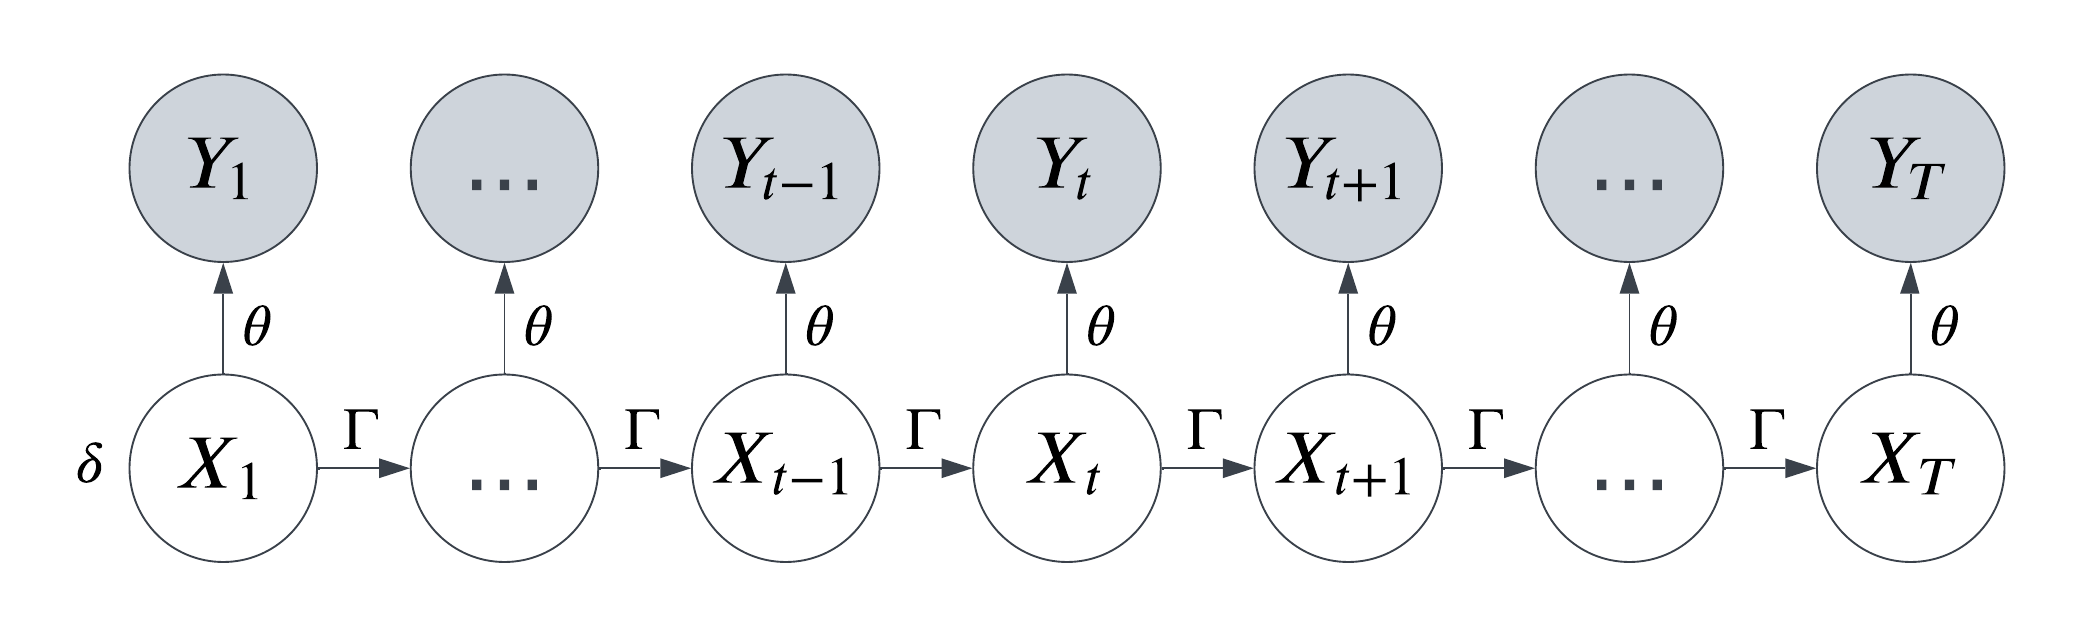
\includegraphics[width=5in]{../plt/HMM.png}
    \caption{Graphical representation of an HMM. $X_t$ corresponds to an unobserved latent state at time $t$ which follows a Markov chain, and $Y_t$ corresponds to an observation at time $t$ that is independent of all other random variables when conditioned on $X_t$.}
    \label{fig:HMM}
\end{figure}

It is convenient to reparameterize the transition probability matrix $\Gamma \in \bbR^{N \times N}$ and initial distribution $\delta \in \bbR^N$ in terms of an auxiliary variable $\eta$ to ensure that all entries are positive and all rows sum to one. One option is to follow the parameterization of \citet{Barajas:2017}:
%
\begin{equation}
    \Gamma^{(i,j)}(\eta) = \frac{\exp(\eta^{(i,j)})}{\sum_{k=1}^N \exp(\eta^{(i,k)})}, \qquad \delta^{(i)}(\eta) = \frac{\exp(\eta^{(i)})}{\sum_{k=1}^N \exp(\eta^{(k)})}
    \label{eqn:reparam}
\end{equation}
%
where $i,j = 1,\ldots,N$ and $\eta^{(i,i)}$ and $\eta^{(1)}$ are set to zero for identifiability. This formulation simplifies likelihood maximization by removing constraints in the optimization problem. One may also incorporate covariates into $\Gamma$ by setting $\eta_t^{(i,j)}(\beta) = \left(\beta^{(i,j)}\right)^T \theta_t$, where $\theta_t$ is a column vector of known covariates and $\beta^{(i,j)}$ is a column vector of unknown regression coefficients. While $\Gamma$ and $\delta$ are functions of $\eta$, we abuse notation in future sections and treat $\Gamma$ and $\delta$ as variables since the mapping is a bijection.

The joint likelihood of some fixed observed data $\bfy$ and given latent states $\bfx$ is
%
\begin{equation}
    p(\bfx,\bfy;\theta,\eta) = \delta^{(x_1)} f^{(x_1)}(y_1; \theta^{(x_1)}) \prod_{t=2}^T \Gamma^{(x_{t-1},x_t)} f^{(x_t)}(y_t; \theta^{(x_t)}).
    \label{eqn:like}
\end{equation}
%
Alternatively, the marginal likelihood of the observed data $\bfy$ alone is 
%
\begin{equation}
    p(\bfy;\theta,\eta) = \delta P(y_1;\theta) \prod_{t=2}^T \Gamma P(y_t;\theta) \mathbf{1}_N.
    \label{eqn:like_marginal}
\end{equation}
%
where $\mathbf{1}_N$ is an $N$-dimensional column vector of ones and $P(y_t;\theta)$ is an $N \times N$ diagonal matrix with the $(i,i)^{th}$ entry $f^{(i)}(y_t; \theta^{(i)})$.

\subsection{Hierarchical Hidden Markov Models}

The transition probability matrix $\Gamma$ can be parameterized to enforce a hierarchical structure \citep{Barajas:2017}. In particular, define a coarse-scale initial distribution $\delta_c \in \bbR^{N_c}$, a coarse-scale probability transition matrix ($\boldsymbol{\Gamma}_c \in \bbR^{{N_c} \times {N_c}}$), ${N_c}$ fine-scale initial distributions $\{\delta_f^{(i)}\}_{i=1}^{N_c}$, each in $\bbR^{N_f^{(i)}}$, and ${N_c}$ fine-scale transition probability matrices $\{\boldsymbol{\Gamma}_f^{(i)}\}_{i=1}^{N_c}$, each in $\bbR^{N_f^{(i)} \times N_f^{(i)}}$. Each initial distribution and probability matrix is parameterized similarly to Equation (\ref{eqn:reparam}). Further, define the matrix $\boldsymbol{\Pi}_f^{(i)}$ as an $N_f^{(i)} \times N_f^{(i)}$ matrix with identical row entries, $\delta_f^{(i)}$, the initial distribution over fine-scale states for the $i^{th}$ coarse-scale state. Then, the global probability transition matrix $\boldsymbol{\Gamma}$ is the following: %\textcolor{red}{I stole this from Vianey}:

\begin{equation} 
\boldsymbol{\Gamma} = 
\begin{pmatrix}
\Gamma_c^{(1,1)}\boldsymbol{\Gamma}_f^{(1)}     & \Gamma_c^{(1,2)} \boldsymbol{\Pi}_f^{(2)}     & \cdots & \Gamma_c^{(1,N_c)}\boldsymbol{\Pi}_f^{(N_c)}  \cr
\Gamma_c^{(2,1)}\boldsymbol{\Pi}_f^{(1)} & \Gamma_c^{(2,2)} \boldsymbol{\Gamma}_f^{(2)}  & \cdots & \Gamma_c^{(2,N_c)}\boldsymbol{\Pi}_f^{(N_c)} \cr
\vdots & \vdots & \ddots & \vdots \cr 
\Gamma_c^{(N_c,1)}\boldsymbol{\Pi}_f^{(1)} & \Gamma_c^{(N_c,2)}\boldsymbol{\Pi}_f^{(2)}      & \cdots & \Gamma_c^{(N_c,N_c)} \boldsymbol{\Gamma}_f^{(N_c)} 
\end{pmatrix}.
\label{exptpm2}
\end{equation}

A model with a transition probability matrix in the form of (\ref{exptpm2}) is known as a hierarchical hidden Markov model, or HHMM. The total number of hidden states for an HHMM is $N = \sum_{i=1}^{N_c} N_f^{(i)}$ and the transition probability matrix $\Gamma$ of a hierarchical HMM is simply a more restricted version of the probability transition matrix from a traditional HMM.

\subsection{State Decoding}

One appealing feature of an HMM is that it is possible to determine the probability distribution of the hidden state at time $t$, $X_t$, conditional of the set of observations $Y_t$. To this end, we define the probability density of the observations between times $s$ and $t$ as $p(y_{s:t};\theta,\eta)$. We also define \textit{forward probabilities} $\alpha^{(i)}_t = p(y_{1:t},X_t = i;\theta,\eta)$ (for $i = 1,\ldots,N$ and $t = 1,\ldots,T$) and \textit{backward probabilities} $\beta^{(i)}_t = p(y_{(t+1):T}|X_t = i;\theta,\eta)$ (for $i = 1,\ldots,N$ and $t = 1,\ldots,T-1$). By convention, $\beta^{(i)}_T = 1$ for $i = 1,\ldots,N$. 
Both $\alpha_t$ and $\beta_t$ can be defined recursively:
%
\begin{align}
    \alpha_1^{(i)}(\theta,\eta) &= \delta^{(i)} f^{(i)}(y_1;\theta), & \alpha_t^{(i)}(\theta,\eta) &= \sum_{j=1}^N \alpha_{t-1}^{(j)} \Gamma^{(j,i)} f^{(i)}(y_t;\theta^{(i)}), \quad t = 2,\ldots,T. \label{eqn:alpha} \\
    %
    \beta_T^{(i)}(\theta,\eta) &= 1, & \beta_t^{(i)}(\theta,\eta) &= \sum_{j=1}^N \Gamma^{(i,j)} f^{(j)}(y_{t+1};\theta) \beta^{(j)}_{t+1}, \quad t = 1,\ldots,T-1. \label{eqn:beta}
\end{align}

We denote the probability that $X_t = i$ given all observations $\bfy$ and parameters $\{\theta,\eta\}$ as $\gamma_t^{(i)}(\theta,\eta)$ for $t = 1,\ldots,T$ and $i = 1,\ldots,N$. Further, we denote the probability that $X_{t-1} = i$ and $X_t = j$ given all observations $\bfy$ and parameters $\{\theta,\eta\}$ as $\xi_t^{(i,j)}(\theta,\eta)$ for $t = 2,\ldots,T$ and $i,j = 1,\ldots,N$. Namely,
%
\begin{gather*}
    \gamma_t^{(i)}(\theta,\eta) = \bbP(X_t = i \mid \bfy ~;~ \theta,\eta), \\ \xi_t^{(i,j)}(\theta,\eta) = \bbP(X_{t-1} = i, X_t = j \mid \bfy ~;~ \theta,\eta). \nonumber
\end{gather*}
%
Both $\gamma_t$ and $\xi_t$ can be calculated from $\alpha_{t-1}$, $\alpha_t$, and $\beta_t$:
%
\begin{gather}
    \gamma_{t}^{(i)}\big(\theta,\eta\big) = \frac{\alpha_{t}^{(i)} ~ \beta_{t}^{(i)}}{\sum_{i'} \alpha_{t}^{(i')} ~ \beta_{t}^{(i')}}, \label{eqn:gamma} \\
    %
    \xi_{t}^{(i,j)}\big(\theta, \eta) = \frac{\alpha_{t-1}^{(i)} ~ \Gamma^{(i,j)} ~ f^{(j)}(y_{t} ~ ; ~\theta) ~ \beta_{t}^{(j)}}{\sum_{i',j'} ~ \alpha_{t-1}^{(i')} ~ \Gamma^{(i',j')}(\eta) ~ f^{(j')}(y_{t} ~ ; ~\theta) ~ \beta_{t}^{(j')}} \label{eqn:xi},
\end{gather}

\subsection{The Baum-Welch Algorithm}

The Baum-Welch algorithm is an optimization technique is used to estimate the parameters of the HMM. It is simply the specific instance of the EM algorithm when applied to HMMs. Suppose a sequence of observations $\bfy$ is observed as output of an HMM with unknown latent states $\bfX$ and unknown parameters $\{\theta,\eta\}$. Define the function $Q(\theta,\eta \mid \theta_{k},\eta_{k})$ as the expected value of the joint log-likelihood $\log p(\bfy,\bfX; \theta,\eta)$ when $\bfX$ is a random variable with density $p(\bfX | \bfy;\theta_{k},\eta_{k})$. The Baum-Welch algorithm updates the parameter estimates at step $k+1$ by maximizing $Q(\theta,\eta \mid \theta_{k},\eta_{k})$ with respect to the parameters $\{\theta,\eta\}$:
%
\begin{gather}
    Q(\theta,\eta \mid \theta_{k},\eta_{k}) \equiv \bbE_{p(\bfX \mid \bfy;\theta_{k},\eta_{k})}\left[\log p(\bfy,\bfX;\theta,\eta) \right]
    \label{eqn:BW_update} \\
    %
    Q^*(\theta_{k},\eta_{k}) \equiv \max_{\theta,\eta}Q(\theta,\eta \mid \theta_{k},\eta_{k}) \\
    %
    \theta^*_{k+1},\eta^*_{k+1} = \argmax_{\theta,\eta} Q(\theta,\eta \mid \theta_{k},\eta_{k})
\end{gather}
%
We can combine Equation (\ref{eqn:BW_update}) with Equation (\ref{eqn:like}) to separate the expected value into three convenient terms:
\begin{align*}
    Q(\theta,\eta \mid \theta_{k},\eta_{k}) &\equiv \bbE_{p(\bfX \mid \bfy;\theta_{k},\eta_{k})}\left[\log p(\bfy,\bfX;\theta,\eta) \right] \\
    &= \bbE_{p(\bfX \mid \bfy;\theta_{k},\eta_{k})} \left[\sum_{t=1}^T \log f^{(X_t)}(y_t;\theta^{(X_t)}) + \log \delta^{(X_1)} + \sum_{t=2}^{T} \log \Gamma^{(X_{t-1},X_{t})} \right] \\
    %
    &= \sum_{t = 1}^T \bbE_{p(\bfX \mid \bfy;\theta_{k},\eta_{k})} \left[ \log f^{(X_t)}(y_t;\theta^{(X_t)})\right]  \\
    & \qquad + \bbE_{p(\bfX \mid \bfy;\theta_{k},\eta_{k})} \Big[\log \delta_{X_1}\Big] + \sum_{t=2}^{T} \bbE_{p(\bfX \mid \bfy;\theta_{k},\eta_{k})} \left[ \log \Gamma^{(X_{t-1},X_{t})} \right] \\
    %
    &= \sum_{t = 1}^T \sum_{i=1}^N \gamma^{(i)}_t(\theta_{k},\eta_{k}) \log f^{(i)}(y_t;\theta^{(i)}) \\
    & \qquad + \sum_{i=1}^N \gamma^{(i)}_1(\theta_{k},\eta_{k}) \log \delta^{(i)} + \sum_{t=2}^{T} \sum_{i=1}^N \sum_{j=1}^N \xi_t^{(i,j)}(\theta_{k},\eta_{k}) \log \Gamma^{(i,j)} 
\end{align*}

Each of the terms on the right-hand side of the equation above only depend upon $\theta$, and $\eta$, respectively. As a result, the maximization problem can be divided into two separate sub-problems. First, we define the functions $F$ and $G$ as follows:
%
\begin{gather}
    F_t(\theta, \theta_k, \eta_k) = - \sum_{i=1}^N \gamma^{(i)}_t(\theta_k, \eta_k) \log f^{(i)}(y_t;\theta), \qquad
    %
    F(\theta, \theta_k,\eta_k) = \frac{1}{T} \sum_{t=1}^T F_t(\theta, \theta_k, \eta_k), \label{eqn:F} \\
    %
    \theta^*_{k+1} = \argmin_{\theta} F(\theta,\theta_k,\eta_k), \label{eqn:EM_update_theta} \\ \nonumber \\
    %
    %
    G_t(\eta, \theta_k, \eta_k) = 
    \begin{cases}
        - \sum_{i=1}^N \gamma^{(i)}_t(\theta_k,\eta_k) \log \delta^{(i)}(\eta), & t = 1, \\\\
        - \sum_{i=1}^N \sum_{j=1}^N \xi^{(i,j)}_t(\theta_k, \eta_k) \log \Gamma^{(i,j)}(\eta), & t \geq 2
    \end{cases}, \qquad
    %
    G(\eta, \theta_k,\eta_k) = \frac{1}{T} \sum_{t=1}^{T} G_t(\eta, \theta_k, \eta_k), \label{eqn:G}\\
    %
    \eta^*_{k+1} = \argmin_{\eta} G(\eta,\theta_k,\eta_k). \label{eqn:EM_update_eta}
\end{gather}
We define $F$ and $G$ such that the M-step of the EM algorithm is a minimization problem to be consistent with existing optimization literature. In addition, note that 
\begin{equation}
   Q(\theta, \eta \mid \theta_{k},\eta_{k}) = -T ~ \left[F(\theta, \theta_k, \eta_k) + G(\eta, \theta_k, \eta_k)\right].
\end{equation}
For notational convenience, we define
\begin{equation}
    F_t^{(k)}(\theta) \equiv F_t(\theta,\theta_k,\eta_k), \quad F^{(k)}(\theta) \equiv F(\theta,\theta_k,\eta_k), \qquad G_t^{(k)}(\eta) \equiv G_t(\eta,\theta_k,\eta_k), \quad G^{(k)}(\eta) \equiv G(\eta,\theta_k,\eta_k).
    \label{eqn:FtGt}
\end{equation}
%
where $F^{(k)}$ and $G^{(k)}$ are random functions. In many simple scenarios the maximization problems above have closed-form solutions. For example, if $\Gamma$ does not depend upon any covariates and $f^{(i)}(y_t;\theta^{(i)})$ is a normal or Poisson probability density function with respect to $y_t$, then the solutions of Equations (\ref{eqn:EM_update_theta}) and (\ref{eqn:EM_update_eta}) are given in Section 4.2 of \citet{Zucchini:2016}. However, in many other situations (e.g. if $\Gamma$ or $f^{(i)}$ depend upon covariates), the maximization problem above is not straightforward and requires numerical maximization techniques. %Whether or not Equations (\ref{eqn:EM_update_theta}) and (\ref{eqn:EM_update_eta}) have closed-form solutions, even defining $F^{(k)}$ and $G^{(k)}$ to initialize the optimization problem (the E-step) has a time cost of $\calO(T)$, which can be expensive for large $T$. 

\iffalse
\subsection{Direct likelihood maximization}

An alternative way to perform inference over HMMs is to directly maximize the marginal likelihood from Equation (\ref{eqn:like_marginal}) using gradient-based optimization techniques. One standard method is gradient descent, which updates $\theta$ or $\eta$ at step $m$ using the following update rule with step sizes $\lambda_F^\eta$ and $\lambda_F^\theta$:
%
\begin{gather}
    \eta_{m+1} = \eta_{m} + \lambda_F^{\eta} \nabla_\eta \log p(\bfy;\theta_{m},\eta_{m}) \\
    %
    \theta_{m+1} = \theta_{m} + \lambda_F^{\theta} \nabla_\theta \log p(\bfy;\theta_{m},\eta_{m}).
    \label{eqn:grad_update}
\end{gather}
%
Using the Fisher identity of the gradient for incomplete data models \citep{Fisher:1925}, the gradient of Equation (\ref{eqn:like_marginal}) can be written as
%
\begin{equation}
    \nabla_{\theta,\eta} \log p(\bfy;\theta,\eta) = \bbE_{p(\bfX \mid \bfy;\theta,\eta)}\left[ \nabla_{\theta,\eta} \log p(\bfy,\bfX;\theta,\eta) \right].
    \label{eqn:fisher_id}
\end{equation}
%
Similarly to the EM algorithm, we can split the gradient of the log-likelihood into separate terms that each depend on only $\theta$ or $\eta$:
%
\begin{gather}
    \nabla_{\theta} \log p(\bfy;\theta,\eta) = \sum_{t=1}^T \sum_{i=1}^N \gamma_t^{(i)}(\theta,\eta) \nabla_{\theta} \log f^{(i)}(y_t;\theta^{(i)}) \label{eqn:theta_update_gd} \\
    %
    \nabla_{\eta} \log p(\bfy;\theta,\eta) = \sum_{i=1}^N \gamma_1^{(i)}(\theta,\eta) \nabla_{\eta} \log \delta^{(i)} + \sum_{t=2}^{T} \sum_{i=1}^N \sum_{j=1}^N \xi_t^{(i,j)}(\theta,\eta) \nabla_{\eta} \log \Gamma^{(i,j)}, \label{eqn:eta_update_gd}
\end{gather}
%
There is a clear connection between the Baum-Welch update from Equation (\ref{eqn:BW_update}) and the gradient given by Equation (\ref{eqn:fisher_id}). In particular, one recovers gradient descent by performing one gradient step within the M-step of the Baum-Welch algorithm rather than solving the entire maximization problem. This connection leads to a natural question: if taking one gradient step within the M- step is equivalent to gradient descent, and solving the M- step entirely results in the Baum-Welch algorithm, then are there other ways to perform the M-step in the EM algorithm with desirable properties? To answer this question, we first review some stochastic optimization techniques.
\fi

\subsection{Stochastic Optimization}

Stochastic optimization techniques can solve minimization problems that can be written as the sum of independent terms, including the one posed in (\ref{eqn:F}) and (\ref{eqn:EM_update_theta}) at step $k$ in the EM algorithm:
%
\begin{equation*}
    \min F^{(k)}(\theta), \qquad F^{(k)}(\theta) = \frac{1}{T}\sum_{t = 1}^T F^{(k)}_t(\theta).
\end{equation*}
%
We focus on optimizing $\theta$ here, but the same logic can be applied to optimizing $\eta$ in (\ref{eqn:G}) and (\ref{eqn:EM_update_eta}).
%
Standard gradient descent updates $\theta$ at step $m$ using the following update rule with step size $\lambda_F$:
%
\begin{equation*}
    \theta_{m+1} = \theta_{m} - \lambda_F \nabla F^{(k)}(\theta_{m}) =  \theta_{m} - \frac{\lambda_F}{T} \sum_{t=1}^T \nabla F^{(k)}_t(\theta_{m}).
\end{equation*}
%
However, this update requires evaluating a gradient for all $t = 1,\ldots,T$, which can be prohibitive if $T$ is large. Alternatively, \citet{Robbins:1951} introduce stochastic gradient descent (or SGD), which updates $\theta$ using an unbiased estimate of the full gradient:
%
\begin{equation*}
    \theta_{m+1} = \theta_{m} - \lambda_F \nabla F^{(k)}_{t_m}(\theta_{m})
\end{equation*}
%
for some $t_m \in \{1,\ldots,T\}$ selected uniformly at random at step $m$. Stochastic gradient descent reduces the amount of time between updates by using an unbiased estimate of the gradient to update $\theta_{m}$. However, the gradient estimates themselves can have high variance, so stochastic gradient descent requires that the step-size $\lambda_F$ decays over time to ensure convergence. In addition, SGD has slower convergence rates compared to full gradient descent \citep{Schmidt:2017}.

Variance-reduced stochastic optimization techniques including (but not limited to) SAG \citep{Schmidt:2017}, SVRG \citep{Johnson:2013}, and SAGA \citep{Defazio:2014} enjoy the speed of stochastic gradient descent as well as the convergence rates of full gradient descent. These algorithms involve storing a table of gradient \textit{estimates} $\widehat \nabla F^{(k)}_t$ that are updated and stored at various stages in the optimization algorithm. The table average then approximates the full gradient $\nabla F^{(k)}(\theta_{m})$. The table of gradient estimates can be used to reduce the variance of future gradient estimates. In particular, SAG uses the update rule:
%
\begin{equation}
    \theta_{m+1} \gets \theta_{m} - \lambda_F \left[\frac{\nabla F^{(k)}_{t_m}(\theta_{m}) - \widehat \nabla F^{(k)}_{t_m}}{T} + \frac{1}{T} \sum_{t=1}^T \widehat \nabla F^{(k)}_{t} \right], \label{eqn:SAG_update}
\end{equation}
%
which is simply the table average with entry $t_m$ updated at step $m$. This update rule is intuitive, but it represents a biased estimate of the gradient $\nabla P(\theta_m)$. This can slow down convergence and makes theoretical analysis of SAG difficult. SVRG and SAGA, on the other hand, utilize an unbiased estimate of the gradient to update $\theta_m$:
%
\begin{equation}
    \theta_{m+1} \gets \theta_{m} - \lambda_F \left[\nabla F^{(k)}_{t_m}(\theta_{m}) - \widehat \nabla F^{(k)}_{t_m} + \frac{1}{T} \sum_{t=1}^T \widehat \nabla F^{(k)}_{t} \right].
    \label{eqn:SAGA_update}
\end{equation}
%
Taking the expected value of the gradient estimate from (\ref{eqn:SAGA_update}) shows that it is unbiased:
%
\begin{align*}
    \bbE\left[\nabla F^{(k)}_{t_m}(\theta_{m}) - \widehat \nabla F^{(k)}_{t_m} + \frac{1}{T} \sum_{t=1}^T \widehat \nabla F^{(k)}_{t} \right] &= \frac{1}{T} \sum_{t=1}^T \nabla F^{(k)}_{t}(\theta_{m}) - \frac{1}{T} \sum_{t=1}^T \widehat \nabla F^{(k)}_{t} + \frac{1}{T} \sum_{t=1}^T \widehat \nabla F^{(k)}_{t} \\
    %
    &= \frac{1}{T} \sum_{t=1}^T \nabla F^{(k)}_{t_m}(\theta_{m}) = \nabla F^{(k)}(\theta_{m}).
\end{align*}
%
After updating the parameters at step $m$, SAG and SAGA simply update the table at position $t_m$: 
%
\begin{equation}
    \widehat \nabla F^{(k)}_{t_m} \leftarrow \nabla F^{(k)}_{t_m}(\theta_{m}).
\end{equation}
%
%After updating the table at position $t_m$ with the SAG/SAGA update rule, the table average $\frac{1}{T} \sum_{t=1}^T \widehat \nabla F^{(k)}_{t}$ must be updated using the previous estimate of $\widehat \nabla F^{(k)}_{t}$. 
Both SAG and SAGA can be memory intensive because the gradient at every index must be stored. On the other hand, SVRG updates the \textit{entire} table average and stores the current parameter estimate $\tilde \theta$ once every $M$ iterations. SVRG then recalculates the table entries $\widehat \nabla F^{(k)}_{t} \equiv \nabla F^{(k)}_{t}(\tilde \theta)$ as needed. As such, SVRG saves memory since it does not store gradient estimates at each index. However, SVRG recalculates table entries at every parameter update, so it can be more computationally expensive than SAGA and SAG. In summary, SVRG is less memory intensive, but more computationally expensive compared to SAGA. This trade-off should be considered by practitioners when deciding between the two algorithms. Algorithm (\ref{alg:SO}) outlines SVRG and SAGA in pseudocode.

\begin{algorithm}
\caption{\texttt{VRSO}$\left(P,z_0,\lambda,K,M\right)$}\label{alg:SO}
\begin{algorithmic}[1]
\Require Loss function $P = \sum_t P_t$, Initial value $z_0$, step size $\lambda$, algorithm (SVRG or SAGA), number of full gradient updates $K$ (classically, $K = 1$ for SAGA), and iterations per full gradient update $M$.
%
\For{$k = 0,\ldots,K-1$}
\State Initialize gradient estimates $\widehat \nabla P_t \leftarrow \nabla P_t (z_k)$ for $t = 1, ..., T.$
\State Initialize $z_{k,0} \leftarrow z_k$.
%
\For{$m = 0,1,\ldots,M-1$}:
    %
    \State Pick $t_{k,m} \in \{1,\ldots,T\}$ uniformly at random.
    %
    \State Update parameters:
    \begin{equation}
        z_{k,m+1} \gets z_{k,m} - \lambda \left[\nabla P_{t_{k,m}}(z_{k,m}) - \widehat \nabla P_{t_{k,m}} + \frac{1}{T} \sum_{t=1}^T \widehat \nabla P_{t} \right]
        \label{eqn:SAGA_update0}
    \end{equation}
    %
    \If{using SAGA}:
    \Comment{update table at index $t_{k,m}$}
        \begin{equation}
            \widehat \nabla P_{t_{k,m}} \leftarrow \nabla P_{t_{k,m}}(z_{k,m}) 
        \end{equation}
    \EndIf
\EndFor
\State $z_{k+1} \gets z_{k,M}$
\EndFor
\State \Return $z_K$
\end{algorithmic}
\end{algorithm}